\subsection{Application for MNIST dataset}
The MNIST database of handwritten digits, available from Yann Lecun's website. MNIST has a training set of 60,000 examples and a test set of 10,000 examples. It is a subset of a larger set available from NIST. The digits have been size-normalized and centred in a fixed-size image. In my test, I'll use 55000 examples from the training set (using Tensorflow datasets). These are $28 \times 28$ images. One way to evaluate the quality of our results is to compare the original data vs the reconstructed ones. 
\begin{figure}[h]
 \centering
 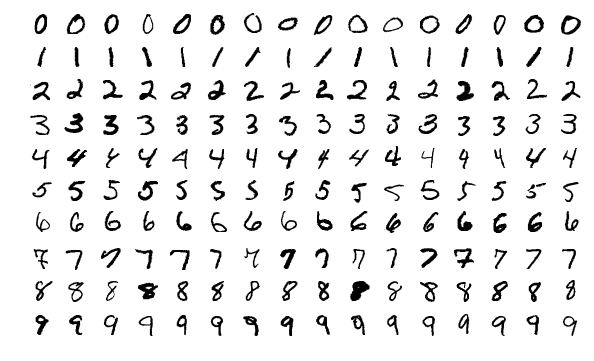
\includegraphics[scale=0.5]{MnistExamples.png}
 % MnistExamples.png: 594x361 px, 72dpi, 20.96x12.74 cm, bb=0 0 594 361
 \caption{Example of MNIST's handwitten digits}
\end{figure}
\subsubsection{Prototype}
My first task is to realise a Sparse Coding prototype to compute Sparse Coding on this dataset, using Python. The aim here is to understand the underlying principles of this method, you can found this prototype in \texttt{Code directory} of this repository as \texttt{SparseCoding.py}. \\
These are some results of this prototype: For time-saving, I used only 100 digits as input.

\subsubsection{SPAMS}
SPAMS (SPArse Modeling Software) is an optimization toolbox for solving various sparse estimation problems.
\begin{itemize}
 \item Dictionary learning and matrix factorization (NMF, sparse PCA, ...)
 \item Solving sparse decomposition problems with LARS, coordinate descent, OMP, SOMP, proximal methods
 \item Solving structured sparse decomposition problems (l1/l2, l1/linf, sparse group lasso, tree-structured regularization, structured sparsity with overlapping groups,...).
\end{itemize}
It is developed and maintained by Julien Mairal (Inria), and contains sparse estimation methods resulting from collaborations with various people: notably, Francis Bach, Jean Ponce, Guillermo Sapiro, Rodolphe Jenatton and Guillaume Obozinski.\\
You can find my code of Sparse Coding/Dictionary Learning on MNIST using SPAMS toolbox on my GitHub \texttt{test\_spams.py}.\\
\newpage
\paragraph{Test 1}
In the first test, I used 256 atoms, 2 000 iterations and $\lambda$ = 0.015 to learn the dictionary and the sparse coefficients. 
w\begin{figure}[h]
 \centering
 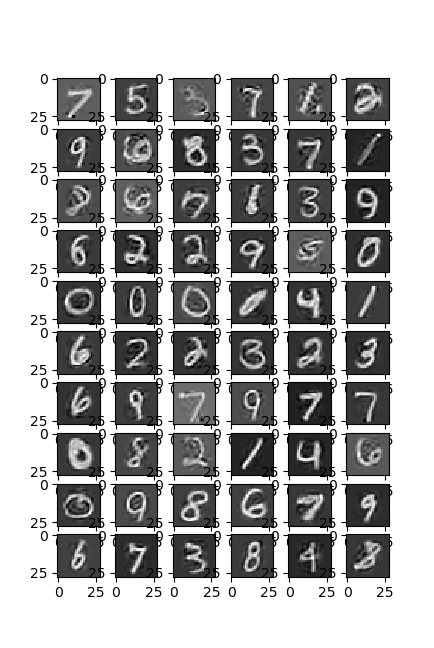
\includegraphics[scale=0.82]{../Results/SPAMS_X_ALL_K256/D.png}
 % D.png: 434x648 px, 100dpi, 11.02x16.46 cm, bb=0 0 312 467
 \caption{Few atoms of D}
\end{figure}

 \begin{figure}[h]
 \begin{subfigure}{.5\textwidth}
 \centering
 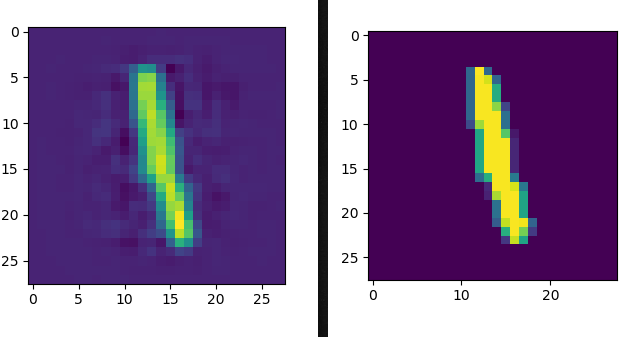
\includegraphics[scale=0.35]{../Results/SPAMS_X_ALL_K256/recons_1.png}
  \caption{Reconstructed 1 vs Original 1}
 % module-capteur-laser.jpg: 600x600 px, 72dpi, 21.17x21.17 cm, bb=0 0 600 600
 \end{subfigure}%
  \begin{subfigure}{.3\textwidth}
 \centering
 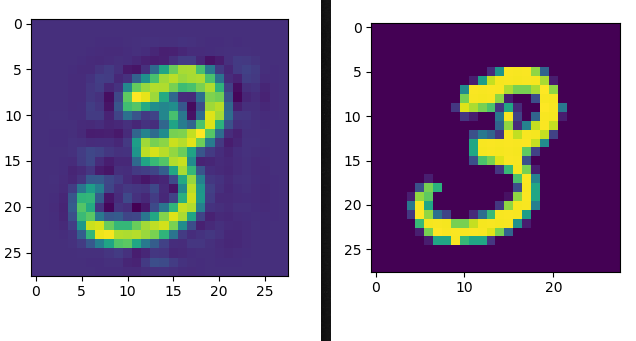
\includegraphics[scale=0.35]{../Results/SPAMS_X_ALL_K256/recons_3.png}
 % module-capteur-laser.jpg: 600x600 px, 72dpi, 21.17x21.17 cm, bb=0 0 600 600
  \caption{Reconstructed 3 vs Original 3}

 \end{subfigure}%
\end{figure}

\newpage

\paragraph{Test 2}In the second test I used 1024 atoms, 1 000 iterations and $\lambda = \frac{1.2}{\sqrt{m}}$ \cite{Mairal:2009:ODL:1553374.1553463} \textit{(In my case $\approx 0.0042857$)}.
\begin{figure}[h]
 \centering
 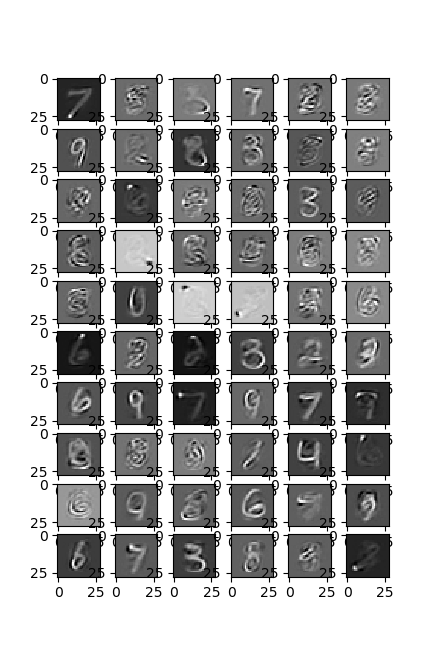
\includegraphics[scale=0.82]{../Results/SPAMS_X_ALL_K1024/D.png}
 % D.png: 1873x1022 px, 100dpi, 47.57x25.96 cm, bb=0 0 1349 736
 \caption{Few atoms of D}
\end{figure}
 \begin{figure}[h]
 \begin{subfigure}{.5\textwidth}
 \centering
 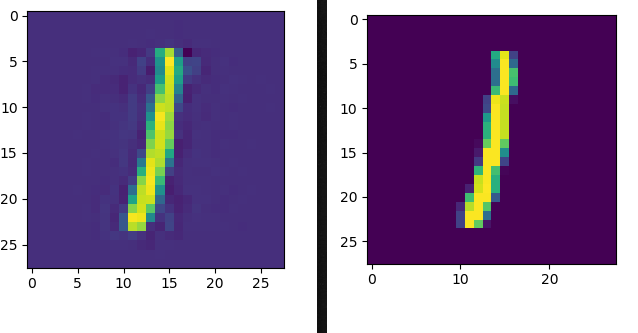
\includegraphics[scale=0.4]{../Results/SPAMS_X_ALL_K1024/lambdaopti_recons1.png}
  \caption{Reconstructed 1 vs Original 1}
 % module-capteur-laser.jpg: 600x600 px, 72dpi, 21.17x21.17 cm, bb=0 0 600 600
 \end{subfigure}%
  \begin{subfigure}{.3\textwidth}
 \centering
 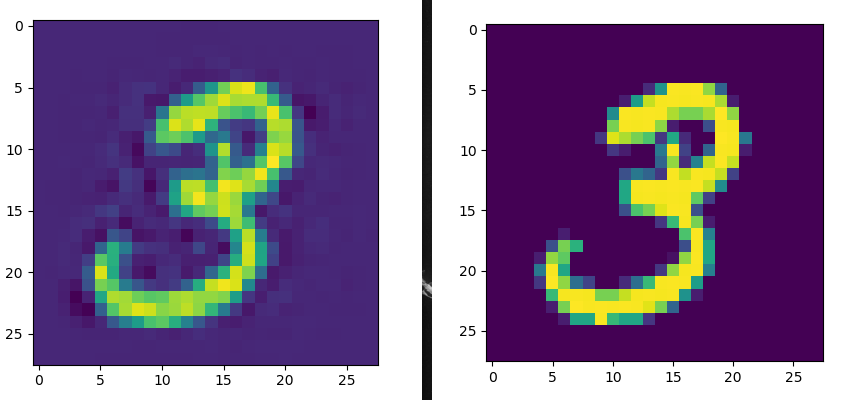
\includegraphics[scale=0.29]{../Results/SPAMS_X_ALL_K1024/lambdaopti_recons3.png}
 % module-capteur-laser.jpg: 600x600 px, 72dpi, 21.17x21.17 cm, bb=0 0 600 600
  \caption{Reconstructed 3 vs Original 3}

 \end{subfigure}%
\end{figure}
\newpage
\paragraph{Test 3} In the third test I used 1024 atoms, 1 000 iterations and $\lambda = 5$.
\begin{figure}[h]
 \centering
 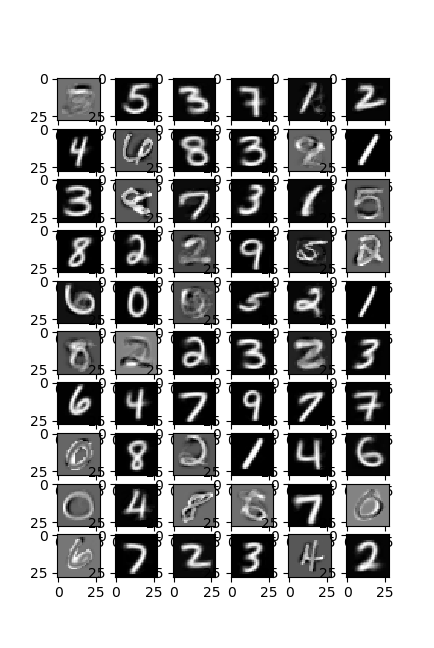
\includegraphics[scale=0.82]{../Results/SPAMS_X_ALL_K1024/D_lambdagrand.png}
 % D_lambdagrand.png: 936x994 px, 100dpi, 23.77x25.25 cm, bb=0 0 674 716
 \caption{Few atoms of D}
\end{figure}

 \begin{figure}[h]
 \begin{subfigure}{.5\textwidth}
 \centering
 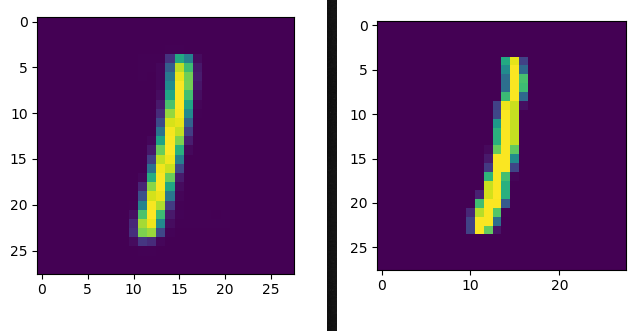
\includegraphics[scale=0.4]{../Results/SPAMS_X_ALL_K1024/lambdagrand_recons1.png}
  \caption{Reconstructed 1 vs Original 1}
 % module-capteur-laser.jpg: 600x600 px, 72dpi, 21.17x21.17 cm, bb=0 0 600 600
 \end{subfigure}%
  \begin{subfigure}{.3\textwidth}
 \centering
 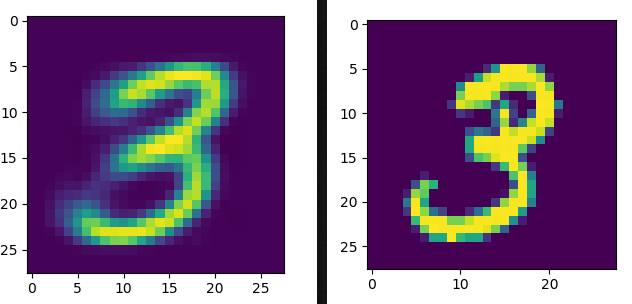
\includegraphics[scale=0.39]{../Results/SPAMS_X_ALL_K1024/lambdagrand_recons3.png}
 % module-capteur-laser.jpg: 600x600 px, 72dpi, 21.17x21.17 cm, bb=0 0 600 600
  \caption{Reconstructed 3 vs Original 3}

 \end{subfigure}%
\end{figure}

\newpage
\paragraph{Test 4} In the fourth test I used 2048 atoms, 1 000 iterations and $\lambda = \frac{1.2}{\sqrt{m}}$
\begin{figure}[h]
 \centering
 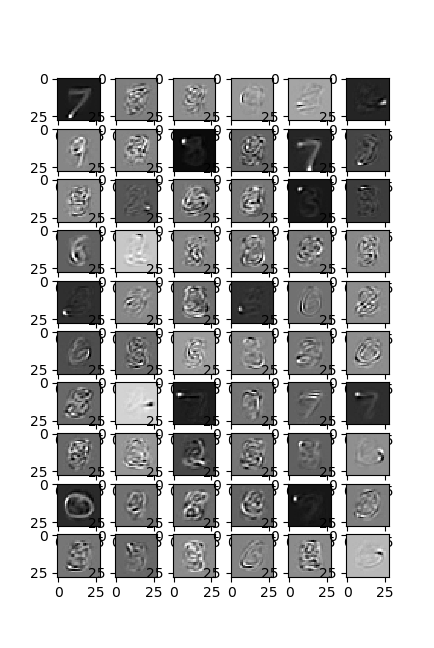
\includegraphics[scale=0.82]{../Results/SPAMS_X_ALL_K_2048/D_K2048.png}
 % D_K2048.png: 936x994 px, 100dpi, 23.77x25.25 cm, bb=0 0 674 716
 \caption{Few atoms of D}
 \end{figure}
 
  \begin{figure}[h]
 \begin{subfigure}{.5\textwidth}
 \centering
 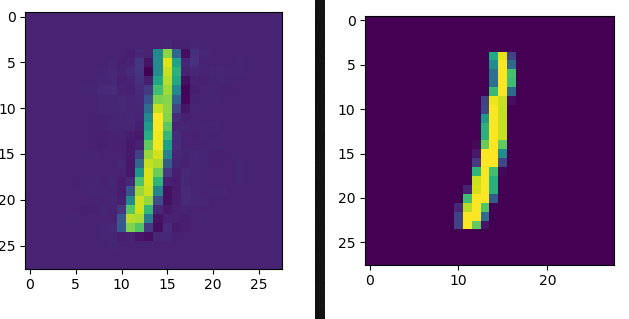
\includegraphics[scale=0.4]{../Results/SPAMS_X_ALL_K_2048/recons1.png}
  \caption{Reconstructed 1 vs Original 1}
 % module-capteur-laser.jpg: 600x600 px, 72dpi, 21.17x21.17 cm, bb=0 0 600 600
 \end{subfigure}%
  \begin{subfigure}{.3\textwidth}
 \centering
 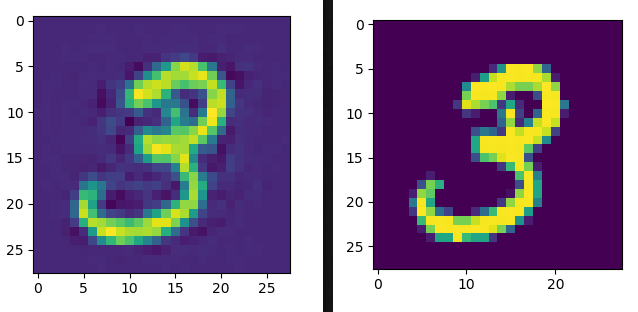
\includegraphics[scale=0.39]{../Results/SPAMS_X_ALL_K_2048/recons3.png}
 % module-capteur-laser.jpg: 600x600 px, 72dpi, 21.17x21.17 cm, bb=0 0 600 600
  \caption{Reconstructed 3 vs Original 3}

 \end{subfigure}%
\end{figure}

\newpage
